% Options for packages loaded elsewhere
\PassOptionsToPackage{unicode}{hyperref}
\PassOptionsToPackage{hyphens}{url}
\PassOptionsToPackage{dvipsnames,svgnames,x11names}{xcolor}
%
\documentclass[
  letterpaper,
  DIV=11,
  numbers=noendperiod]{scrartcl}
\usepackage{amsmath,amssymb}
\usepackage{lmodern}
\usepackage{iftex}
\ifPDFTeX
  \usepackage[T1]{fontenc}
  \usepackage[utf8]{inputenc}
  \usepackage{textcomp} % provide euro and other symbols
\else % if luatex or xetex
  \usepackage{unicode-math}
  \defaultfontfeatures{Scale=MatchLowercase}
  \defaultfontfeatures[\rmfamily]{Ligatures=TeX,Scale=1}
\fi
% Use upquote if available, for straight quotes in verbatim environments
\IfFileExists{upquote.sty}{\usepackage{upquote}}{}
\IfFileExists{microtype.sty}{% use microtype if available
  \usepackage[]{microtype}
  \UseMicrotypeSet[protrusion]{basicmath} % disable protrusion for tt fonts
}{}
\makeatletter
\@ifundefined{KOMAClassName}{% if non-KOMA class
  \IfFileExists{parskip.sty}{%
    \usepackage{parskip}
  }{% else
    \setlength{\parindent}{0pt}
    \setlength{\parskip}{6pt plus 2pt minus 1pt}}
}{% if KOMA class
  \KOMAoptions{parskip=half}}
\makeatother
\usepackage{xcolor}
\IfFileExists{xurl.sty}{\usepackage{xurl}}{} % add URL line breaks if available
\IfFileExists{bookmark.sty}{\usepackage{bookmark}}{\usepackage{hyperref}}
\hypersetup{
  colorlinks=true,
  linkcolor={blue},
  filecolor={Maroon},
  citecolor={Blue},
  urlcolor={Blue},
  pdfcreator={LaTeX via pandoc}}
\urlstyle{same} % disable monospaced font for URLs
\usepackage{longtable,booktabs,array}
\usepackage{calc} % for calculating minipage widths
% Correct order of tables after \paragraph or \subparagraph
\usepackage{etoolbox}
\makeatletter
\patchcmd\longtable{\par}{\if@noskipsec\mbox{}\fi\par}{}{}
\makeatother
% Allow footnotes in longtable head/foot
\IfFileExists{footnotehyper.sty}{\usepackage{footnotehyper}}{\usepackage{footnote}}
\makesavenoteenv{longtable}
\usepackage{graphicx}
\makeatletter
\def\maxwidth{\ifdim\Gin@nat@width>\linewidth\linewidth\else\Gin@nat@width\fi}
\def\maxheight{\ifdim\Gin@nat@height>\textheight\textheight\else\Gin@nat@height\fi}
\makeatother
% Scale images if necessary, so that they will not overflow the page
% margins by default, and it is still possible to overwrite the defaults
% using explicit options in \includegraphics[width, height, ...]{}
\setkeys{Gin}{width=\maxwidth,height=\maxheight,keepaspectratio}
% Set default figure placement to htbp
\makeatletter
\def\fps@figure{htbp}
\makeatother
\setlength{\emergencystretch}{3em} % prevent overfull lines
\providecommand{\tightlist}{%
  \setlength{\itemsep}{0pt}\setlength{\parskip}{0pt}}
\setcounter{secnumdepth}{-\maxdimen} % remove section numbering
\KOMAoption{captions}{tableheading}
\makeatletter
\makeatother
\makeatletter
\@ifpackageloaded{caption}{}{\usepackage{caption}}
\AtBeginDocument{%
\renewcommand*\contentsname{Table of contents}
\renewcommand*\listfigurename{List of Figures}
\renewcommand*\listtablename{List of Tables}
\renewcommand*\figurename{Figure}
\renewcommand*\tablename{Table}
}
\@ifpackageloaded{float}{}{\usepackage{float}}
\floatstyle{ruled}
\@ifundefined{c@chapter}{\newfloat{codelisting}{h}{lop}}{\newfloat{codelisting}{h}{lop}[chapter]}
\floatname{codelisting}{Listing}
\newcommand*\listoflistings{\listof{codelisting}{List of Listings}}
\makeatother
\makeatletter
\@ifpackageloaded{caption}{}{\usepackage{caption}}
\@ifpackageloaded{subcaption}{}{\usepackage{subcaption}}
\makeatother
\makeatletter
\makeatother
\ifLuaTeX
  \usepackage{selnolig}  % disable illegal ligatures
\fi

\author{}
\date{}

\begin{document}

\hypertarget{sec-intro}{%
\section{Introduction}\label{sec-intro}}

In section Section~\ref{sec-intro}

\hypertarget{sec-method}{%
\section{Methodological background}\label{sec-method}}

Counterfactual search happens in the feature space: we are interested in
understanding how we need to change individual attributes in order to
change the model output to a desired value or label
\cite{molnar2020interpretable}. Typically the underlying methodology is
presented in the context of binary classification:
\(M: \mathcal{X} \mapsto y\) where and \(y\in\{0,1\}\). Let \(t=1\) be
the target class and let \(\overline{x}\) denote the factual feature
vector of some individual outside of the target class, so
\(\overline{y}=M(\overline{x})=0\). Then the counterfactual search
objective originally proposed by \cite{wachter2017counterfactual} is as
follows

\begin{equation}\protect\hypertarget{eq-obj}{}{
\min_{\underline{x} \in \mathcal{X}} h(\underline{x}) \ \ \ \mbox{s. t.} \ \ \ M(\underline{x}) = t
}\label{eq-obj}\end{equation}

where \(h(\cdot)\) quantifies how complex or costly it is to go from the
factual \(\overline{x}\) to the counterfactual \(\underline{x}\). To
simplify things we can restate this constrained objective
(Equation~\ref{eq-obj}) as the following unconstrained and
differentiable problem:

\begin{equation}\protect\hypertarget{eq-solution}{}{
\underline{x} = \arg \min_{\underline{x}}  \ell(M(\underline{x}),t) + \lambda h(\underline{x})
}\label{eq-solution}\end{equation}

Here \(\ell\) denotes some loss function targeting the deviation between
the target label and the predicted label and \(\lambda\) governs the
stength of the complexity penalty. Provided we have gradient access for
the black-box model \(M\) the solution to this problem
(Equation~\ref{eq-solution}) can be found through gradient descent. This
generic framework lays the foundation for most state-of-the-art
approaches to counterfactual search and is also used as the baseline
approach in \texttt{CounterfactualExplanations}.

That being said, numerous extensions of this simple approach have been
developed since counterfactual explanations were first proposed in 2017
(see \cite{verma2020counterfactual} and \cite{karimi2020survey} for
surveys). The various approaches largely differ in how they define the
complexity penalty. In \cite{wachter2017counterfactual}, for example,
\(h(\cdot)\) is defined in terms of the Manhattan distance between
factual and counterfactual feature values. While this is an intuitive
choice, it is too simple to address many of the desirable properties of
effective counterfactual explanations that have been set out. These
desiderata include: \textbf{closeness} -the average distance between
factual and counterfactual features should be small
(\cite{wachter2017counterfactual}); \textbf{actionability} - the
proposed feature perturbation should actually be actionable
(\cite{ustun2019actionable}, \cite{poyiadzi2020face});
\textbf{plausibility} - the counterfactual explanation should be
plausible to a human (\cite{joshi2019towards}); \textbf{unambiguity} - a
human should have no trouble assigning a label to the counterfactual
(\cite{schut2021generating}); \textbf{sparsity} - the counterfactual
explanation should involve as few individual feature changes as
possible; \textbf{robustness} - the counterfactual explanation should be
robust to domain and model shifts (\cite{upadhyay2021towards});
\textbf{diversity} - ideally multiple diverse counterfactual
explanations should be provided (\cite{mothilal2020explaining}); and
\textbf{causality} - counterfactual explanations reflect the structual
causal model underlying the data generating process
(\cite{karimi2020algorithmic},\cite{karimi2021algorithmic}).

\hypertarget{using-counterfactualexplanations}{%
\section{\texorpdfstring{Using
\texttt{CounterfactualExplanations}}{Using CounterfactualExplanations}}\label{using-counterfactualexplanations}}

\hypertarget{counterfactual-generators}{%
\subsection{Counterfactual generators}\label{counterfactual-generators}}

\begin{figure}

{\centering 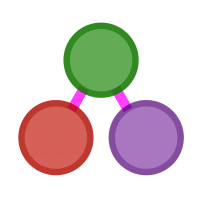
\includegraphics{./juliagraphs.png}

}

\caption{Figure}

\end{figure}

\hypertarget{empirical-example}{%
\section{Empirical example}\label{empirical-example}}

\hypertarget{related-and-future-work}{%
\section{Related and future work}\label{related-and-future-work}}

\end{document}
